\documentclass[10pt]{article}
\usepackage[margin=1in]{geometry}
\usepackage{graphicx}
\usepackage{hyperref}
\usepackage{amsmath}
\usepackage{amssymb}
\usepackage{booktabs}
\usepackage{caption}
\usepackage{subcaption}
\usepackage{xcolor}

% Figure spacing
\setlength{\intextsep}{12pt plus 2pt minus 2pt}
\setlength{\floatsep}{12pt plus 2pt minus 2pt}
\setlength{\textfloatsep}{12pt plus 2pt minus 2pt}

% Caption formatting
\captionsetup{font=small,labelfont=bf,labelsep=period,skip=6pt}

\hypersetup{
    colorlinks=true,
    linkcolor=blue,
    urlcolor=blue,
    citecolor=blue
}

\title{\textbf{Scoring Matters: A Reproducible NEDC Evaluation of SeizureTransformer on TUSZ}}

\author{
John H. Jung, MD, MS\\
Independent Researcher\\
\texttt{jj@novamindnyc.com}
}

\date{}

\begin{document}

\maketitle

\begin{abstract}
Claims about deep learning model performance in seizure detection are difficult to verify without standardized evaluation protocols. We report the first evaluation of SeizureTransformer on the Temple University Hospital EEG Seizure Corpus (TUSZ) using the Neureka EEG Data Consortium (NEDC) v6.0.0 scoring tools—the same evaluation framework used in peer-reviewed literature for two decades. At the paper's published parameters (threshold=0.8, kernel=5, duration=2.0s), we measure 26.89 false alarms per 24 hours (FA/24h) at 45.63\% sensitivity using NEDC's any-overlap (OVERLAP) scoring—27 times higher than the 1 FA/24h reported on the proprietary Dianalund dataset. The discrepancy grows to 137-fold (136.73 FA/24h) with time-aligned event scoring (TAES). We demonstrate that scoring methodology alone produces a 15.9-fold difference in reported false alarm rates: identical predictions yield 136.73 FA/24h (NEDC TAES), 26.89 FA/24h (NEDC OVERLAP), and 8.59 FA/24h (SzCORE Event). Parameter tuning for the clinical target of 10 FA/24h achieves only 33.90\% sensitivity—far below the 75\% required for clinical use. Our comprehensive analysis includes 865 TUSZ recordings (258,173 minutes), parameter sweeps across 180 configurations, and three standardized scoring methodologies. We provide complete evaluation infrastructure enabling reproducible benchmarking of seizure detection algorithms. These findings highlight the critical importance of standardized evaluation in medical AI, where methodological choices can mask order-of-magnitude performance differences.
\end{abstract}

\section{Introduction}

The evaluation of seizure detection algorithms suffers from a fundamental reproducibility crisis. Published models report dramatically different performance metrics while claiming state-of-the-art results, yet these claims often cannot be verified due to proprietary datasets, missing evaluation code, or ambiguous scoring definitions. This opacity particularly affects deep learning approaches, where complex architectures and extensive hyperparameter spaces compound the verification challenge.

SeizureTransformer exemplifies this problem. The model reports 80.30\% sensitivity at 1.0 FA/24h on a proprietary Danish dataset (Dianalund), with no public evaluation possible. While the authors released model weights—a commendable step toward reproducibility—the absence of standardized evaluation on public datasets leaves critical questions unanswered about real-world performance.

We present, to our knowledge, the first evaluation of SeizureTransformer on TUSZ's held-out test set using Temple's NEDC v6.0.0 scoring software. Our systematic comparison evaluates identical model predictions using three scoring methodologies: NEDC TAES (time-aligned event scoring), NEDC OVERLAP (binary any-overlap), and SzCORE Event. At the paper's default parameters (threshold=0.8, kernel=5, duration=2.0s), we observe 45.63\% sensitivity at 26.89 FA/24h with NEDC OVERLAP—a 27-fold increase from the Dianalund benchmark claim. The same predictions yield 136.73 FA/24h with NEDC TAES (137-fold increase) and 8.59 FA/24h with SzCORE Event. This 3.1-fold difference between NEDC OVERLAP and SzCORE Event stems entirely from scoring methodology, independent of model architecture or parameters.

\begin{figure}[h]
\centering
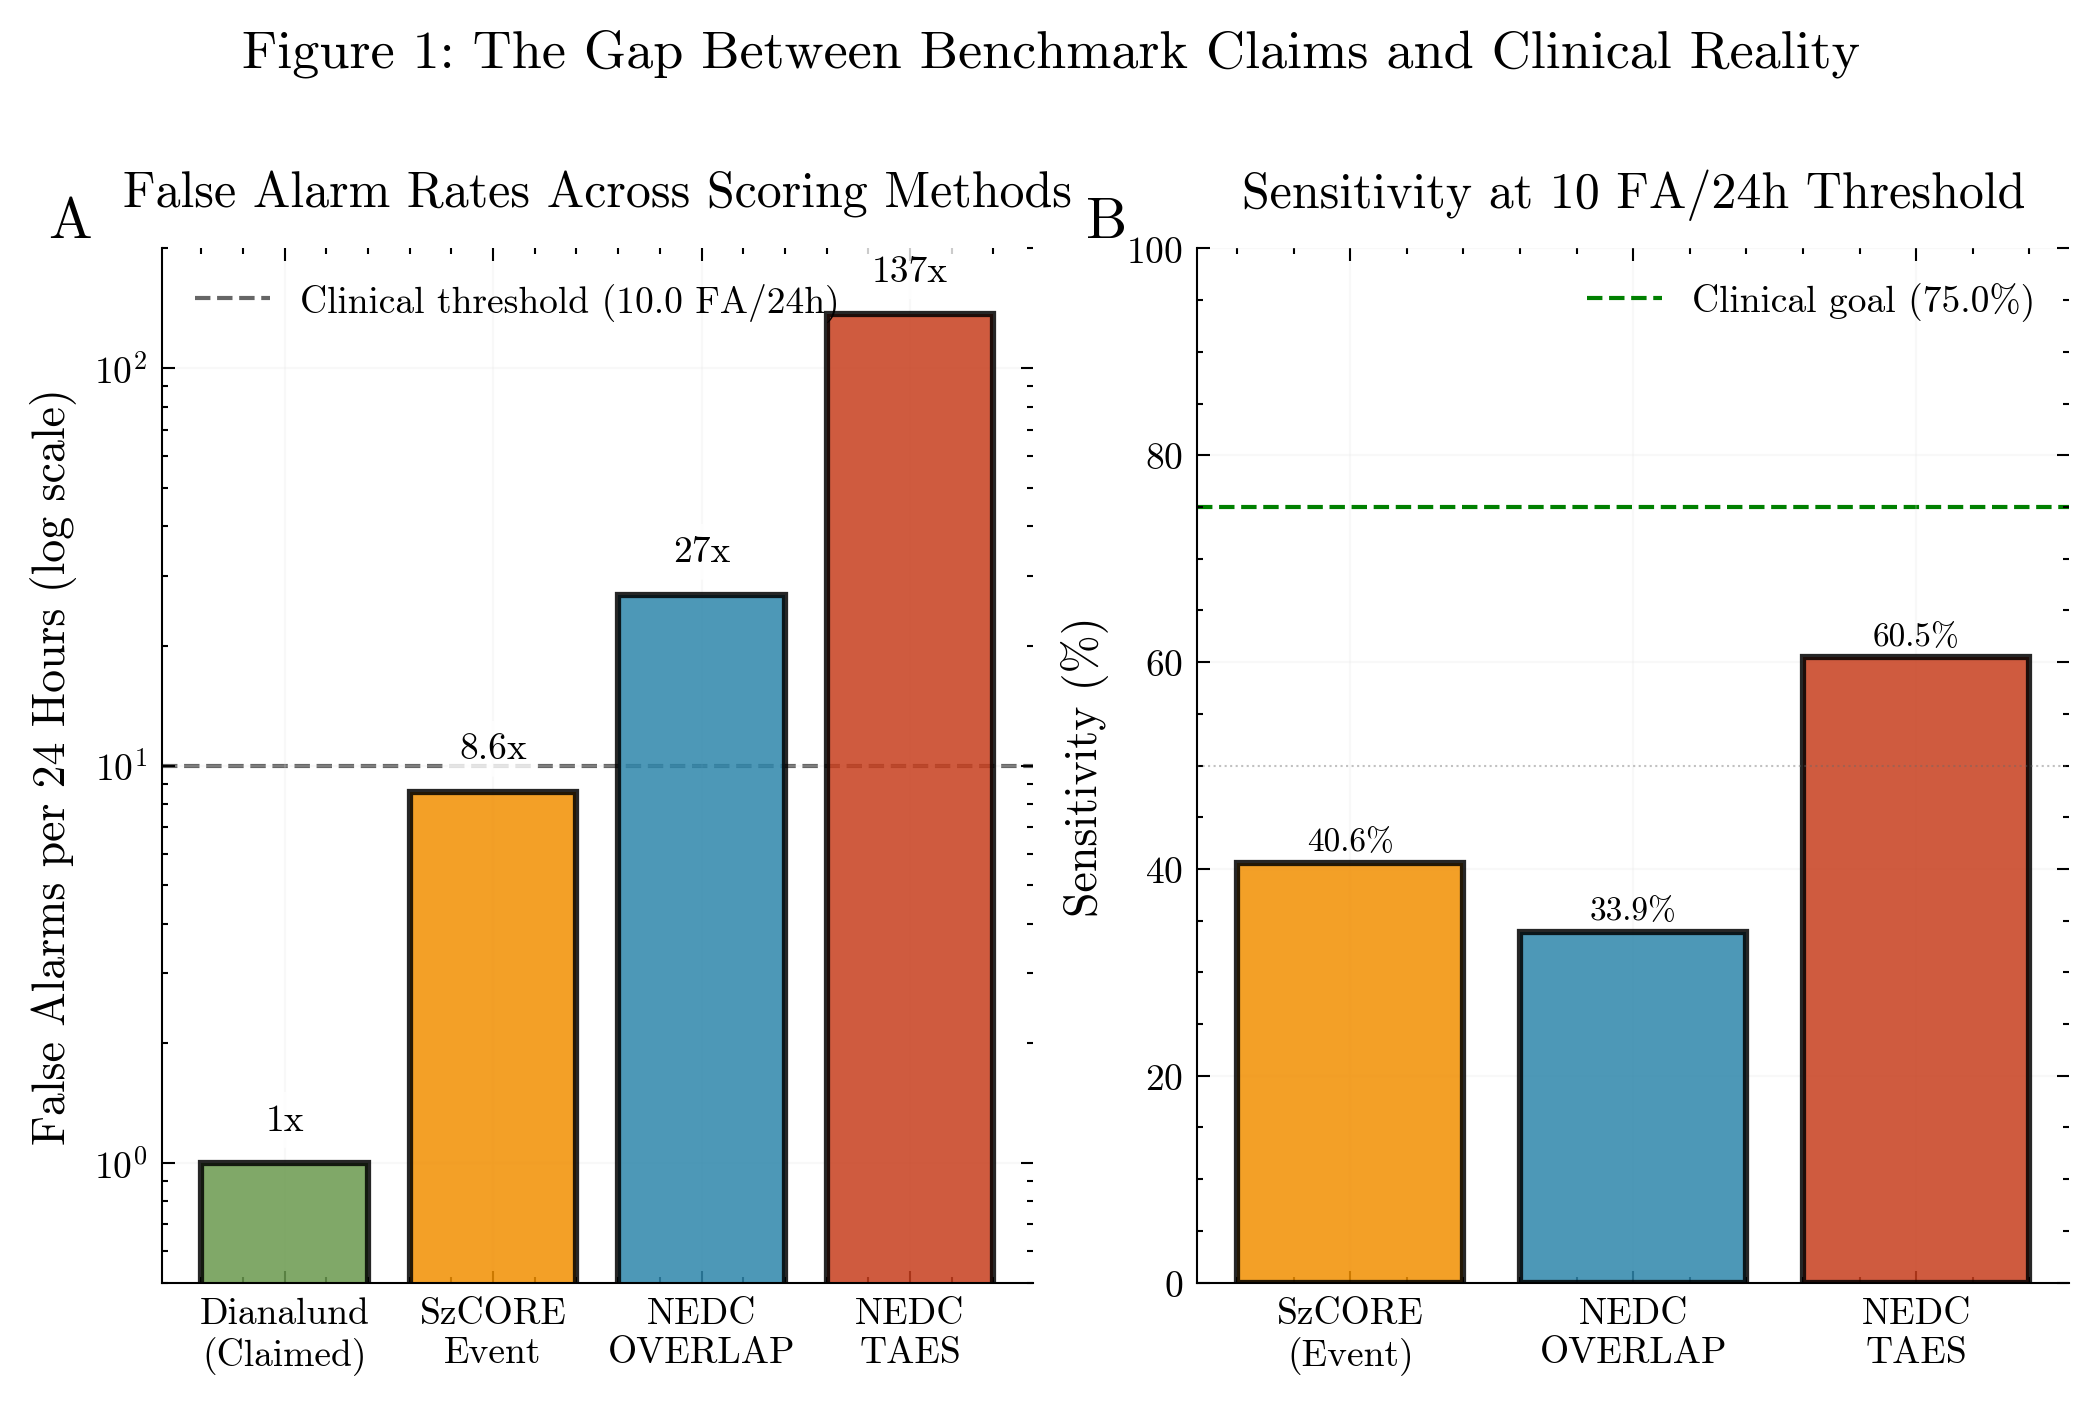
\includegraphics[width=\textwidth]{figures/output/arxiv/fig1_performance_gap.png}
\caption{Performance gap visualization showing the 27–137x difference between claimed and measured false alarm rates. Panel A shows false alarm rates on a logarithmic scale, comparing Dianalund's claimed performance (1 FA/24h) against our TUSZ evaluation using different scoring methods. Panel B displays sensitivity near 10 FA/24h using each scorer's closest available operating point (no interpolation). SzCORE Event uses any-overlap with clinical tolerances (-30 s/+60 s; merge <90 s, split >5 min).}
\label{fig:performance-gap}
\end{figure}

Our contributions extend beyond revealing performance gaps. We provide: (1) a reproducible NEDC v6.0.0 evaluation pipeline for TUSZ, bridging the research-to-clinic evaluation gap; (2) comprehensive operating points for clinical deployment, including evaluation at a clinically-motivated threshold of <=10 FA/24h; (3) quantitative evidence that scoring methodology alone can account for multi-fold performance differences, highlighting the critical need for transparent reporting; and (4) open-source infrastructure enabling the community to replicate and extend our evaluation framework. When optimizing for the 10 FA/24h threshold, SeizureTransformer achieves only 33.90\% sensitivity with NEDC OVERLAP, falling far short of the 75\% sensitivity goal for clinical systems.

\end{document}